\section{习题参考答案}
\subsection*{一、填空}
\begin{enumerate}
    \item 选无穷远处为电势零点,半径为$R$的导体球带电后,其电势为$V_0$,则球外离球心距离为$r$~($r>R$)~处的电场强度的大小为\anl{$E=\frac{RV_0}{r^2}$},球内离球心距离$r(r<R)$处的电势$U$=\anl{$V_0$}.
    \begin{note}
        \textcolor{red}{具体如下:}
        \begin{figure}[H]
            \centering
            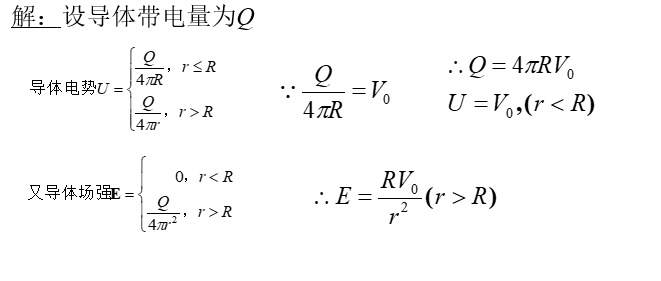
\includegraphics[width=0.45\textheight]{ans39}
        \end{figure}
    \end{note}
    \item 半径为$R$的金属球与地连接,在与球心$O$相距$d$处有一电荷为$q$的点电荷,如图所示~\ref{Fig:59}。设地的电势为零,则球上的感应电荷在球心$O$点处产生的电势$U_0$=\anl{$-\frac{q}{4\pi \varepsilon_0 r}$}.    
    \begin{figure}[H]
        \centering
        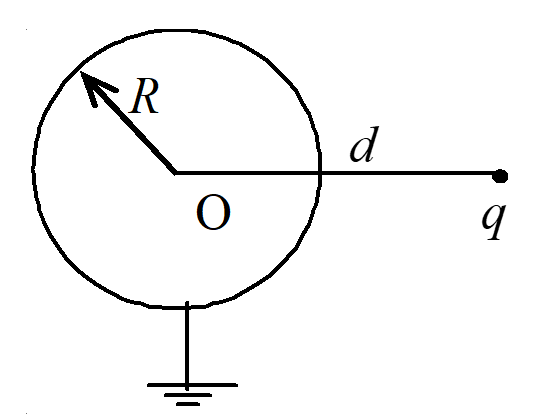
\includegraphics[width=0.25\textwidth]{fig59}
        \caption{如图所示}\label{Fig:59}
    \end{figure}
    \begin{note}
        \textcolor{red}{导体接地,所以导体电势为0. 导体在球心的电势为感应电荷在球心的电势与点电荷在球心的电势的叠加。 $0=U_0+\frac{q}{4\pi \varepsilon_0 r}$
        }
    \end{note}
    \item 一孤立带电导体球,其表面处场强的方向垂直于导体表面,当把另一带电体放在这个导体球附近时,该导体球表面处场强的方向\anl{垂直导体表面}.
    \item 在两板间距为$d$的平行板电容器中,平行地插入一块厚度为$d/2$的金属大平板,则电容变为原来的\anl{$2C_0$} 倍;如果插入的是厚度为$d/2$的相对电容率为$\varepsilon_r = 4$的大介质平板,则电容变为原来的\anl{$1.6C_0$} 倍.
    \begin{note}
        \textcolor{red}{具体如下:}
        \begin{figure}[H]
            \centering
            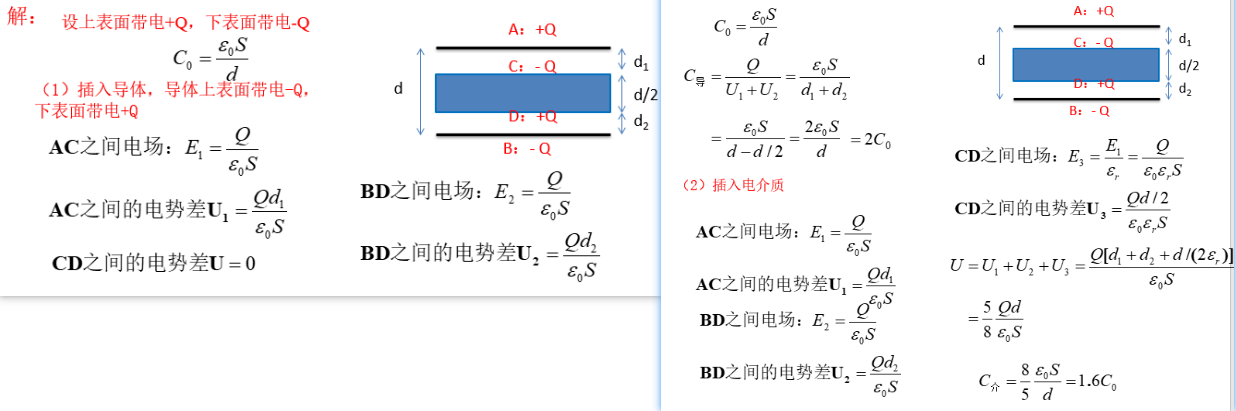
\includegraphics[width=0.55\textheight]{ans40}
        \end{figure}
    \end{note}
    \item 一平行板电容器两极板间电压为$U$,其间充满相对电容率为$\varepsilon_r$的各向同性均匀电介质,电介质厚度为$d$。则电介质中的电场能量密度$W_e$=\anl{$\frac{1}{2}\varepsilon_0\varepsilon_r(\frac{U}{d})^2$}.
    \begin{note}
        $W_e=\frac{1}{2}\varepsilon_0\epsilon_r E^2=\frac{1}{2}\varepsilon_0\varepsilon_r(\frac{U}{d})^2$
    \end{note}
    \item 一平行板电容器二极板间充满相对介电常数$\epsilon_r$的电介质,则电容变为原来的\underline{\makebox[3em]{$\varepsilon_r$}}倍.
    \item 真空中两块互相平行的无限大均匀带电平面。其电荷密度分别为$+\sigma$和$+2\sigma$,两板之间的距离为$d$,两板间的电场强度大小$E$=\anl{$\frac{\sigma}{2\varepsilon_0}$}.
    \begin{note}
        \textcolor{red}{两板之间的电场为两个无限大带电平面电场叠加, 上板电场$E_1= \sigma/2\varepsilon_0$,方向向下.\ \ 下板电场$E_2= 2\sigma/2\varepsilon_0$,方向向上
        两板之间的电场方向向上大小$E=E_2-E_1 = \sigma/2\varepsilon_0.$
        }
    \end{note}
    \item 电荷$q_1$、$q_2$、$q_3$和$q_4$在真空中的分布如图所示~\ref{Fig:60}, 
    其中~$q_2$~是半径为R的均匀带电球体, $S$为闭合曲面,
    则通过闭合曲面$S$的电通量$\displaystyle{\oiint_S {\vec{E}\cdot \mathrm{d}\vec{S}}}$=\anl{$(q_1+q_2)/\varepsilon_0$}.
    \begin{figure}[H]
        \centering
        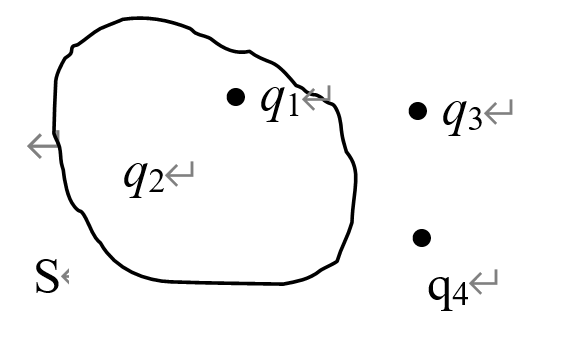
\includegraphics[width=0.25\textwidth]{fig60}
        \caption{如图所示}\label{Fig:60}
    \end{figure}
    \item 真空中一半径为$R$的均匀带电球面,总电量为~$Q~(Q>0)$。今在球面上挖去非常小块的面积 $\Delta S$(连同电荷),且假设不影响原来的电荷分布。则挖去$\Delta S$后,球心处电场强度的大小$E$=\anl{$\frac{\Delta SQ}{16\pi^2 \varepsilon_0 r^4}$}.
    \begin{note}
        \textcolor{red}{具体如下:}
        \begin{figure}[H]
            \centering
            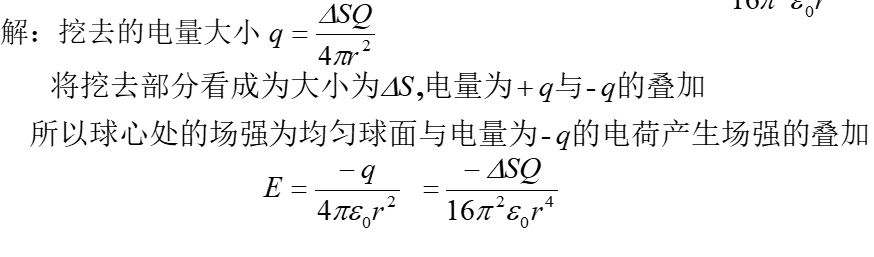
\includegraphics[width=0.55\textheight]{ans41}
        \end{figure}
    \end{note}
\end{enumerate}
\subsection*{二、选择}
\begin{enumerate}
    \item  在一个孤立的导体球壳内,若在偏离球中心处放一个点电荷,则在球壳内、外表面上将出现感应电荷,其分布将是~\anss{B}
    \twoch{内表面均匀,外表面也均匀.}{内表面不均匀,外表面均匀.}{内表面均匀,外表面不均匀.}{内表面不均匀,外表面也不均匀.}
    \begin{note}
        \textcolor{red}{内表面不均匀是为保证导体内部电场为零;\ \ 内部场强为零,要求外表面电荷均匀分布,此时外表面电荷在内部产生场强为零,否则,在内部一定产生电场,无法保证导体中场强为零。
        }
    \end{note}
    \item 对于处在静电平衡下的导体,下面的叙述中,正确的是~\anss{A}
    \onech{导体内部无净电荷,电荷只能分布在导体表面}{导体表面上各处的面电荷密度与表面紧邻处的电场强度的大小成反比}{孤立的导体处于静电平衡时,表面各处的面电荷密度与各处表面的曲率成反比}{沿导体表面移动点电荷,静电场力做功}
    \begin{note}
        \textcolor{red}{B:正比 \ \ C:正比\ \ D:不做功}
    \end{note}
    \item 一带正电荷的物体$M$,靠近一不带电的金属导体$N$,$N$的左端感应出负电荷,右端感应出正电荷,若将N的左端接地,如图所示~\ref{Fig:61},则~\anss{B}
    \twoch{$N$上的负电荷入地}{$N$上的正电荷入地}{$N$上的电荷不动}{$N$上所有电荷都入地}
    \begin{figure}[H]
        \centering
        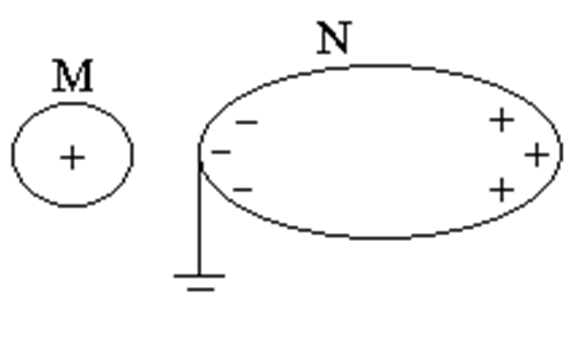
\includegraphics[width=0.25\textwidth]{fig61}
        \caption{如图所示}\label{Fig:61}
    \end{figure}
    \begin{note}
        \textcolor{red}{解 :接地的作用只有一个,就是使导体电势为零。带正电的物体放在导体旁边,这部分正电荷对导体的电势贡献为正,则必须有另一部分电荷对导体的电势贡献为负,这部分电荷就是导体上的感应负电荷。因此接地后导体上留下来的是负电荷,入地的是正电荷。故选B
        }
    \end{note}
    \item 两个带电不等的金属球,直径相等,但一个是空心,一个是实心的。现使它们互相接触,则这两个金属球上的电荷~\anss{B}
    \fourch{不变化}{平均分配}{空心球电量多}{实心球电量多}
    \begin{note}
        \textcolor{red}{解 :两个球接触,电荷密度相等。
        因为两金属球是导体,电荷分布在表面。所以面密度相等。直径相等,所以表面积相等。所以两球的电荷相等。故选B
        }
    \end{note}
    \item 将一个试验电荷$q_0$~(正电荷)~放在带有负电荷的大导体附近~$p$~点处,测得它所受的力的大小为~$F$,若考虑到电量$q_0$不是足够小, 则~\anss{A}
    \onech{$F/q_0$~比~$p$~点处原先的场强数值大}{ $F/q_0$~比$p$点处原先的场强数值小}{$F/q_0$等于原先$p$点处场强数值}{$F/q_0$与$p$点处场强数值关系无法确定}
    \begin{note}
        \textcolor{red}{解:若$q_0$不是足够小,则能影响到大导体的电荷分布。$q_0$带正电,导体带负电。\ 所以导体靠近$q_0$处负电荷分布多一点。\ 所以$q_0$受到导体的电场力要大一些。
        }
    \end{note}
    \item 一平板电容器始终与端电压一定的电源相联,当电容器两极板间为真空时,电场强度为$\vec{E_0}$,电位移为~$\vec{D_0}$,而当极板间充满相对电容率为$\varepsilon_r$的各向同性均匀电介质时,电场强度为$\vec{E}$,电位移为$\vec{D}$,则~\anss{B}
    \twoch{$\vec{E}$=$\vec{E_0}/\varepsilon_r$, $\vec{D}=\vec{D_0}$}{$\vec{E}$=$\vec{E_0}$, $\vec{D}=\varepsilon_r\vec{D_0}$}{$\vec{E}$=$\vec{E_0}/\varepsilon_r$, $\vec{D}=\vec{D_0}/\varepsilon_r$}{$\vec{E}$=$\vec{E_0}$, $\vec{D}=\vec{D_0}$}
    \begin{note}
        \textcolor{red}{具体如下:}
        \begin{figure}[H]
            \centering
            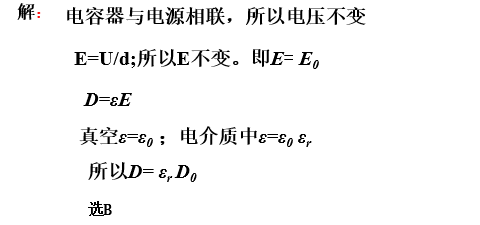
\includegraphics[width=0.55\textheight]{ans42}
        \end{figure}
    \end{note}
    \item 关于有电介质存在时的高斯定理,下列说法正确的是~\anss{C}
    \onech{高斯面内不包围自由电荷,则面上各点电位移矢量$\vec{D}$为零}{高斯面上$\vec{D}$处处为零,则面内必不存在自由电荷}{高斯面的$\vec{D}$通量仅与面内自由电荷有关}{高斯面的$\vec{D}$通量为零,则面内必不存在自由电荷}
    \begin{note}
        \textcolor{red}{A:错,电位移矢量的通量为0; B:错,存在自由电荷(正电荷等于负电荷)。D:错,存在自由电荷(正电荷等于负电荷) 
        }
    \end{note}
    \item 用力$F$把电容器中的电介质板拉出, 在图(a)和图(b)的两种情况下,电容器中储存的静电能量将~\anss{D}
    \fourch{都增加}{都减少}{(a)增加,(b)减小}{(a)减少,(b)增加}
    \begin{note}
        \textcolor{red}{解: 将电介质拉出,电容$C$变小。未断电源, $U$不变,所以$Q$减小,$W=(1/2)~UQ$ 减小,  所以(a)减小;
        断电源,$Q$不变,所以$U$增大,$W=(1/2)UQ$增大, 所以(b)增大。
        }
    \end{note}
    \item 一个平行板电容器,充电后与电源断开,当用绝缘手柄将电容器两极板间距离减小,则两极板间的电势差、电场强度的大小$E$ 、电场能量$W$将发生如下变化~\anss{A}
    \twoch{$U_{12}$~减小,$E$~不变,$W$~减小}{$U_{12}$~增大,$E$~增大,$W$~增大}{$U_{12}$~增大,$E$~不变,$W$~增大}{$U_{12}$~减小,$E$~减小,$W$~不变}
    \begin{note}
        \textcolor{red}{具体如下:}
        \begin{figure}[H]
            \centering
            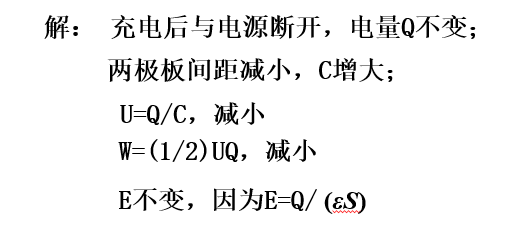
\includegraphics[width=0.35\textheight]{ans43}
        \end{figure}
    \end{note}
    \item 半径分别$R$和$r$的两个球导体~($R>r$)~相距很远,今用细导线把它们连接起来,使两导体带电,电势为$U_0$,则两球表面的电荷面密度之比$\sigma_R/\sigma_r$为~\anss{B}
    \fourch{$R/r$}{$r/R$}{$R^2/r^2$}{$1$}
    \begin{note}
        \textcolor{red}{具体如下:}
        \begin{figure}[H]
            \centering
            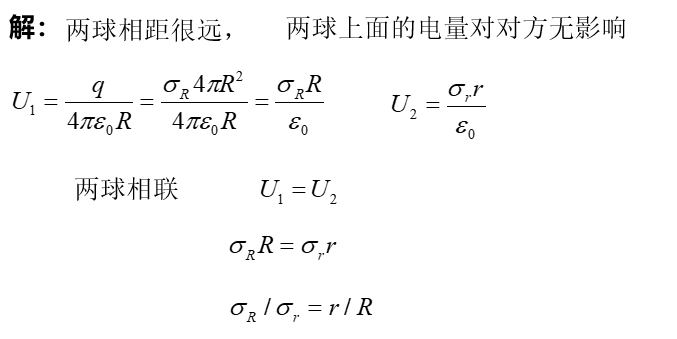
\includegraphics[width=0.35\textheight]{ans44}
        \end{figure}
    \end{note}
    \item 有一电荷$q$及金属导体$A$,且$A$处在静电平衡状态,则~\anss{C}
    \onech{导体内$E=0$,$q$不在导体内产生场强;}{导体内$E\neq 0$,$q$在导体内产生场强;}{导体内$E=0$,$q$在导体内产生场强;}{导体内$E\neq 0$,$q$不在导体内产生场强.}
    \item 平行板电容器在接入电源后,把两板间距拉大,则电容器~\anss{D}
    \twoch{电容增大}{电场强度增大}{所带电量增大}{电容、电量及两板内场强都减小}
    % \begin{note}
    %     \textcolor{red}{$E=\frac{U}{d}, C=\frac{\varepsilon S}{d}, Q=CU$, $U$不变, $d=CU$}
    % \end{note}
\end{enumerate}
\subsection*{三、计算题}
\begin{enumerate}
    \item 如图~\ref{Fig:62},点电荷~$Q$~放在导体球壳的中心,球的内、外半径分别为$a$和$b$,求场强和电势分布.
    \begin{figure}[H]
        \centering
        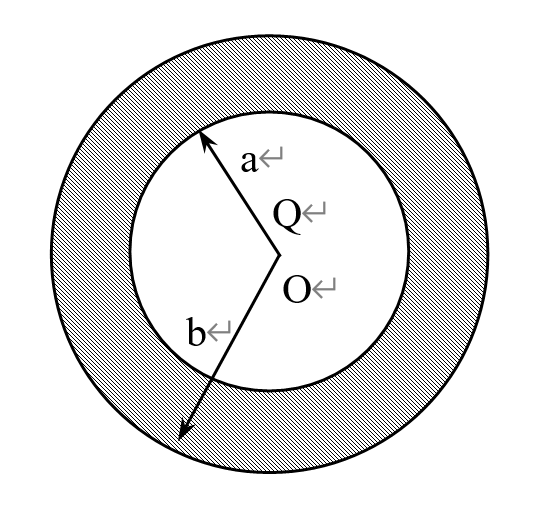
\includegraphics[width=0.3\textwidth]{fig62}
        \caption{如图所示}\label{Fig:62}
    \end{figure}
    \vspace*{0.5cm}
    \begin{solution}
        如图:
        \begin{figure}[H]
            \centering
            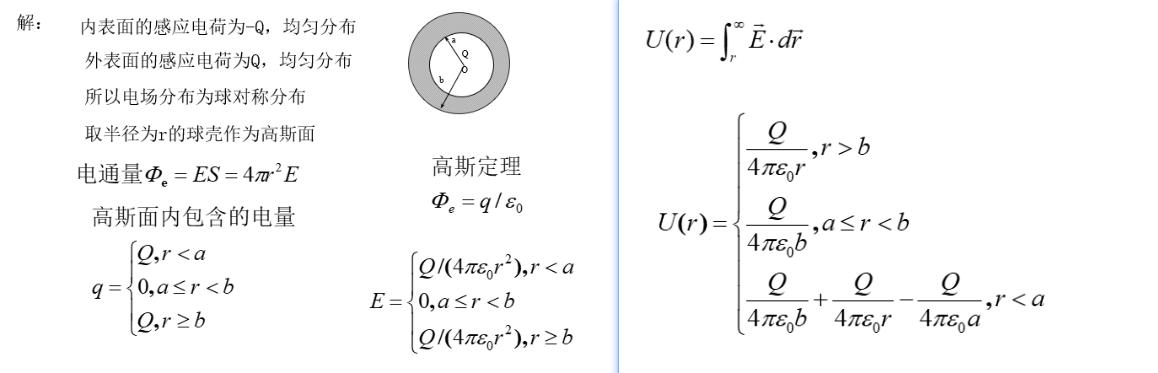
\includegraphics[width=0.58\textheight]{ans45}
        \end{figure}
    \end{solution}
    \item 一球形电容器,内球壳半径为$R_1$外球壳半径为$R_2$,两球壳间充满了相对电容率为$\varepsilon_r$的各向同性均匀电介质,设两球壳间电势差为$U_{12}$,求:
    \begin{enumerate}[label=(\arabic*)]
        \item 电容器的电容;
        \item 电容器储存的能量。
    \end{enumerate}
    \begin{solution}
        如图:
        \begin{figure}[H]
            \centering
            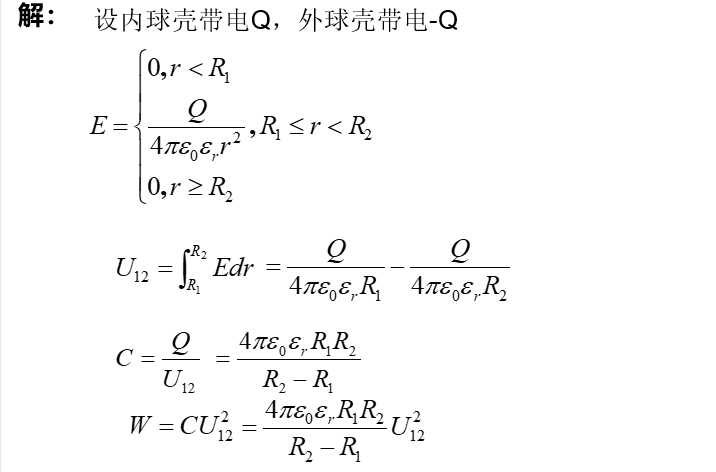
\includegraphics[width=0.55\textheight]{ans46}
        \end{figure}
    \end{solution}
    \item 如图~\ref{Fig:63},半径为$R_1$的导体球带正电$Q_1$,球外有一同心导体球壳,其内外半径分别为$R_2$和$R_3$,球壳带正电$Q_2$,求:
    \begin{enumerate}[label=(\arabic*)]
        \item 此带电系统的场强分布;
        \item 球的电势$U_1$和球壳的电势$U_2$;
        \item 球与球壳的电势差;
        \item 若用导线将球和球壳相连,$U_1$和$U_2$分别为多少?
    \end{enumerate}
    \begin{figure}[H]
        \centering
        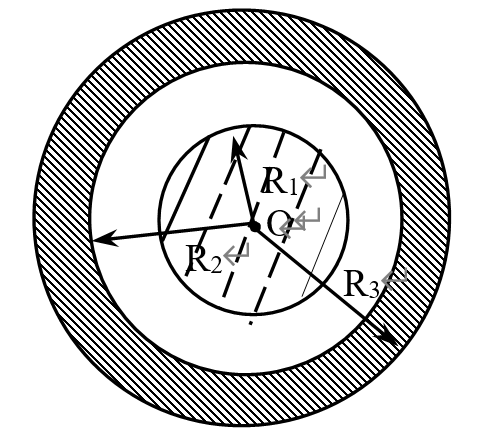
\includegraphics[width=0.25\textwidth]{fig63}
        \caption{如图所示}\label{Fig:63}
    \end{figure}
    \begin{solution}
        如图:
        \begin{figure}[H]
            \centering
            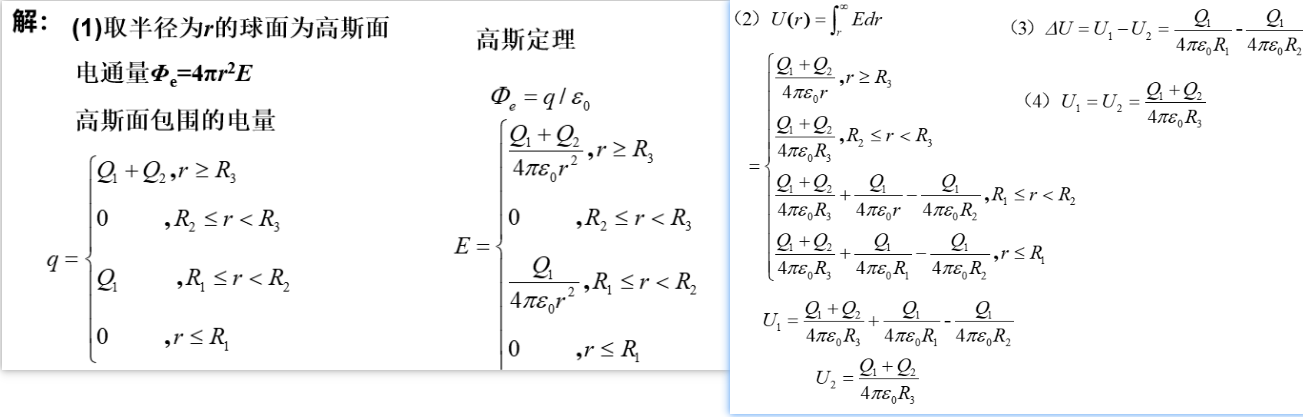
\includegraphics[width=0.59\textheight]{ans47}
        \end{figure}
    \end{solution}
    \item 如图~\ref{Fig:64},一平行板电容器,其极板面积为$S$,间距为$d$,中间有两层厚度各为$d_1$和$d_2$,相对电容率分别为$\varepsilon_{r1}$和$\varepsilon_{r2}$的电介质层(且$d_1+d_2=d$)。两极板上自由电荷面密度分别为$±\sigma$,求
    \begin{enumerate}[label=(\arabic*)]
        \item 两介质层中的电位移和电场强度;
        \item 极板间的电势差;
        \item 电容
    \end{enumerate}
    \begin{figure}[H]
        \centering
        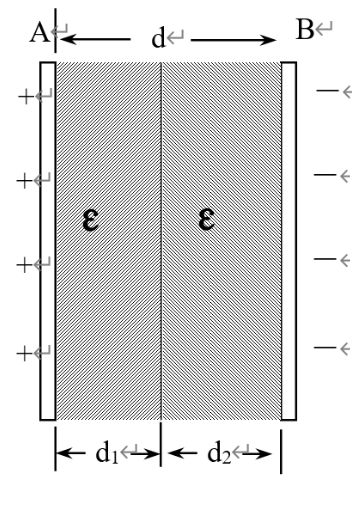
\includegraphics[width=0.25\textwidth]{fig64}
        \caption{如图所示}\label{Fig:64}
    \end{figure}
    \begin{solution}
        如图:
        \begin{figure}[H]
            \centering
            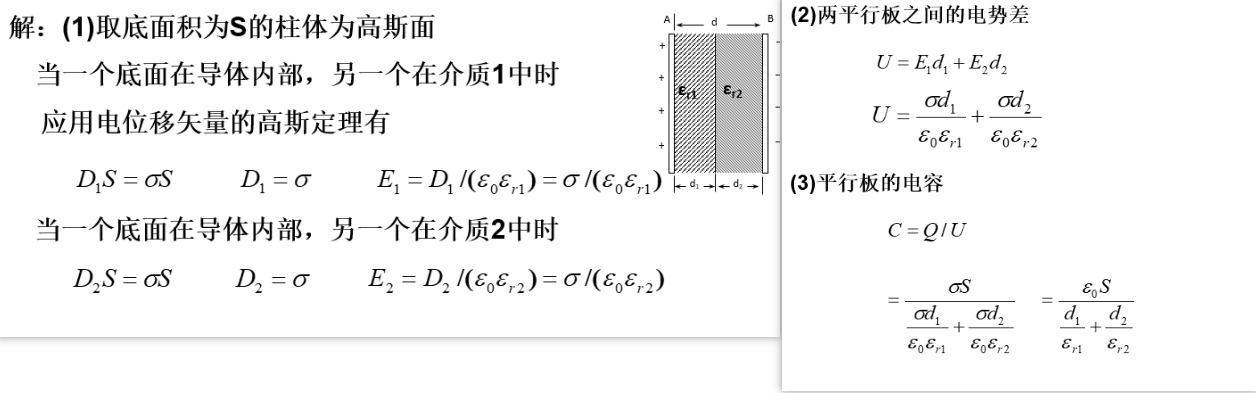
\includegraphics[width=0.55\textheight]{ans48}
        \end{figure}
    \end{solution}
\end{enumerate}